%----------------------------------------------------------------------------------------
%	PACKAGES AND OTHER DOCUMENT CONFIGURATIONS
%----------------------------------------------------------------------------------------

\documentclass[final,hyperref={pdfpagelabels=false}]{beamer}

\usepackage[orientation=portrait,size=a0,scale=1.3]{beamerposter} % Use the beamerposter package for laying out the poster with a portrait orientation and an a0 paper size

\usetheme{I6pd2} % Use the I6pd2 theme supplied with this template

\usepackage[utf8]{inputenc}
\usepackage[english]{babel} % English language/hyphenation
\usepackage{lipsum}
\usepackage{amsmath,amsthm,amssymb,latexsym} % For including math equations, theorems, symbols, etc
%\usepackage{subcaption}
\usepackage[export]{adjustbox}

%\usefonttheme[onlymath]{serif} % Uncomment to use a Serif font within math environments

%\boldmath % Use bold for everything within the math environment

\usepackage{booktabs} % Top and bottom rules for tables
\usepackage[]{units}
\usepackage{siunitx}
\usepackage{wrapfig}
\usepackage{ragged2e}
\usepackage{changepage}
\usepackage{csquotes}
\usepackage{hyperref}
\usepackage{cleveref}
%\usepackage{natbib}
%\usepackage{subcaption}

\setbeamertemplate{bibliography entry title}{}
\setbeamertemplate{bibliography entry location}{}
\setbeamertemplate{bibliography entry note}{}
\renewcommand{\baselinestretch}{1.1}

\graphicspath{{fig/}} % Location of the graphics files

%\usecaptiontemplate{\small\structure{\insertcaptionname~\insertcaptionnumber: }\insertcaption} % A fix for figure numbering

\title{\LARGE Fast generative models on an accelerated\linebreak{} neuromorphic physical model system} % Poster title

\author{\normalsize A.~F.~Kungl\textsuperscript{1,2}, A.~Baumbach\textsuperscript{1,2}, S.~Schmitt\textsuperscript{1}, J.~Kl\"ahn\textsuperscript{1}, N.~G\"urtler\textsuperscript{1}, P.~M\"uller\textsuperscript{1}, D.~Dold\textsuperscript{1,2}, A.~Kugele\textsuperscript{1}, L.~Leng\textsuperscript{1,2}, E.~M\"uller\textsuperscript{1}, C.~Koke\textsuperscript{1}, M.~Kleider\textsuperscript{1}, C.~Mauch\textsuperscript{1}, O.~J.~Breitwieser\textsuperscript{1}, M.~G\"uttler\textsuperscript{1}, D.~Husmann\textsuperscript{1}, K.~Husmann\textsuperscript{1}, A.~Hartel\textsuperscript{1}, V.~Karasenko\textsuperscript{1},  J.~Ilmberger\textsuperscript{1}, A.~Gr\"ubl\textsuperscript{1},  J.~Schemmel\textsuperscript{1}, K.~Meier\textsuperscript{1}, M.~A.~Petrovici\textsuperscript{1,2} } % Author(s)

\institute{\small \textsuperscript{1}Heidelberg University, Kirchhoff-Institute for Physics; \textsuperscript{2}University of Bern, Institute for Physiology} % Institution(s)

%----------------------------------------------------------------------------------------
%	FOOTER TEXT
%----------------------------------------------------------------------------------------

\newcommand{\leftfoot}{\url{http://www.kip.uni-heidelberg.de/vision/publications/}} % Left footer text

\newcommand{\rightfoot}{fkungl@kip.uni-heidelberg.de} % Right footer text

%----------------------------------------------------------------------------------------

\begin{document}
	\newcommand{\blockSpaceOne}{\vspace{1.3cm}}
\newcommand{\interBlockSpaceOne}{\vspace{1.5cm}}
\newcommand{\blockSpaceTwo}{\vspace{1.3cm}}
\newcommand{\interBlockSpaceTwo}{\vspace{.95cm}}
\newcommand{\secondBlockImSpace}{\vspace{.25cm}}
\newcommand{\thirdBlockImSpace}{\vspace{1.125cm}}

\begin{frame} % The whole poster is enclosed in one beamer frame
	\vspace{-.5cm}
	\begin{columns}
		\begin{column}{.005\textwidth}\end{column}

		
		\begin{column}{0.99\textwidth}
			\begin{columns}[t]

				\begin{column}{.01\textwidth}\end{column}

				\begin{column}{0.32\textwidth}


					\begin{block}{\large 1 The Bayesian brain}
					\blockSpaceOne


					\justifying
					\begin{adjustwidth}{1.cm}{1.cm}
					 The noisy behavior of cortical neurons might be a hallmark of an underlying stochastic computation scheme.
					 Such a scheme would enable the brain to cope with ambiguous inputs and offers an explanation for behavioral effects like bistable images (duck/rabbit) as sampling from different modes of a posterior distribution.
					 The \textbf{neural sampling hypothesis} \cite{fiser2010statistically} proposes that some cortical areas implement \textbf{sampling-based Bayesian inference}.

					\end{adjustwidth}

					\thirdBlockImSpace
					\vspace{0.49cm}
					\begin{center}
						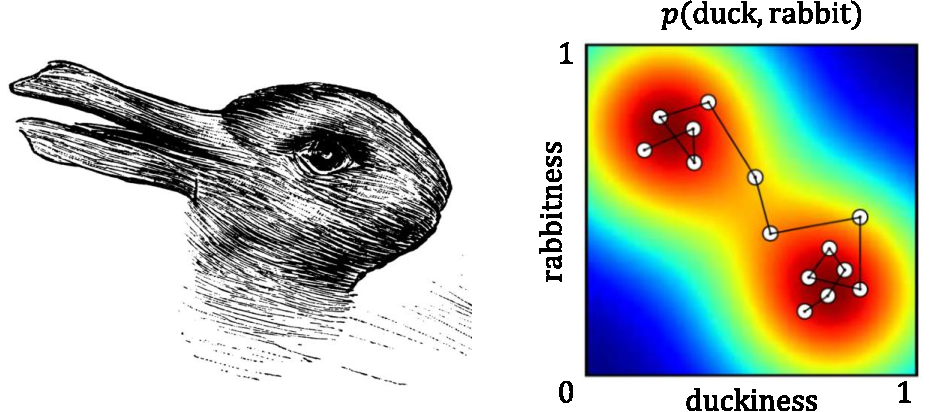
\includegraphics[width=0.8\textwidth]{rabbitDuck}
					\end{center}
					\vspace{0.49cm}
					\thirdBlockImSpace

					\begin{adjustwidth}{1cm}{1cm}
					
					These models are of particular interest for physical model systems, which face similar challenges as the brain.
					\textbf{We review two works \cite{dold2019stochasticity,kungl2019accelerated}, in which we deployed stochastic spiking networks as robust and flexible models on  analog neuromorphic hardware.}

					\end{adjustwidth}

					\blockSpaceOne
					\end{block}


					\interBlockSpaceOne



					\begin{block}{\large 2 Sampling with spikes}
					\blockSpaceOne

					\begin{adjustwidth}{1.cm}{1.cm}
					\justifying
					For applications on spiking hardware, we require models that explicitly treat and use spiking neural networks.

					\thirdBlockImSpace					\begin{center}
						\includegraphics[width=.9\textwidth]{figTHfull}
					\end{center}
					\thirdBlockImSpace

					In the \textbf{LIF sampling} framework \cite{petrovici2016stochastic} a single neuron describes a binary random variable based on its spiking behavior (Fig-A-B).
					Immediately after a spike the neuron is in the \emph{on-state} and otherwise in the \emph{off-state}.
					The network approximately samples from a Boltzmann distribution over binary random variables $z_i$:
					\thirdBlockImSpace
					\begin{equation}
					p(z) \sim \frac{1}{Z} \exp \left ( \frac{1}{2} \sum_{ij} W_{ij} z_i z_j + \sum_{i} b_i z_i  \right)
					\end{equation}
					\thirdBlockImSpace
					\end{adjustwidth}
					This framework establishes an imporant connection to Boltzmann machines.
					For practical applications we use a \textbf{hierarchical sampling network} (Fig-C) inspired by restricted Boltzmann machines \cite{hinton1984boltzmann}.



					\blockSpaceOne
					\end{block}


				\end{column}

				\begin{column}{.01\textwidth}\end{column}

				\begin{column}{0.32\textwidth}


					\begin{block}{\large 3 Deterministic sampling}
					\blockSpaceOne

					\begin{adjustwidth}{1.cm}{1.cm}
					\justifying
					In most models of cortical networks, temporal variability is introduced using explicit white noise sources.
					This is, however, problematic because i) the \textbf{background activity of other brain areas is not necessarily white noise} and ii) a neuromorphic implementation would require dedicated, uncorrelated noise sources for every neuron. 
					\end{adjustwidth}

					\thirdBlockImSpace
					\begin{center}
						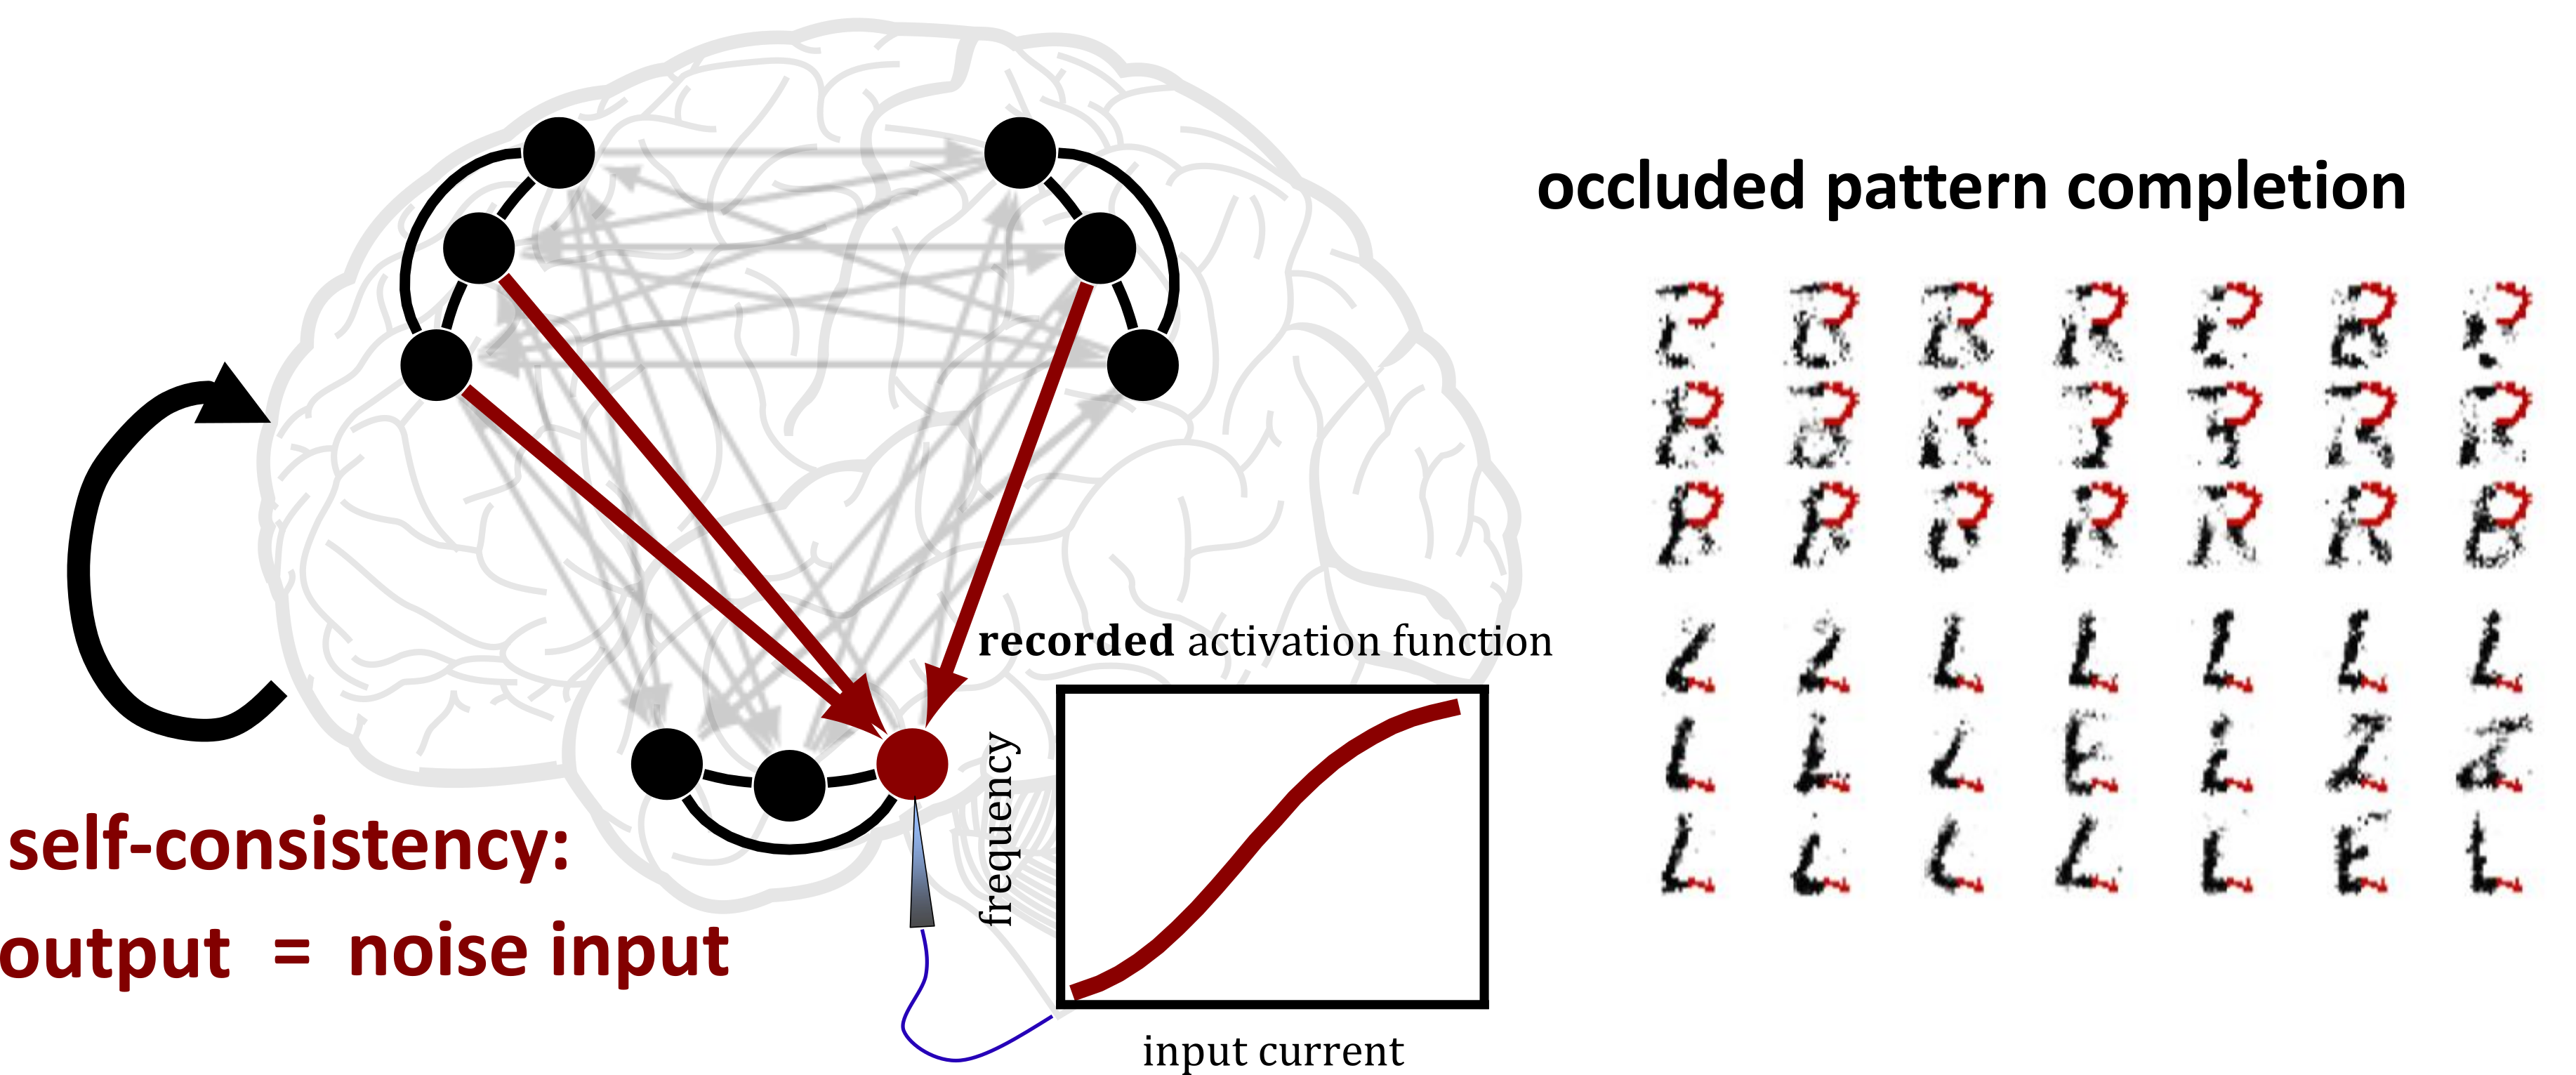
\includegraphics[width=.9\textwidth]{noisybrain.png}
					\end{center}
					\thirdBlockImSpace

					\begin{adjustwidth}{1.cm}{1.cm}
					\justifying

					We  found \cite{dold2019stochasticity} that \textbf{an  ensemble  of  dynamically  fully  deterministic,  but functionally probabilistic networks} can learn a connectivity pattern that enables probabilistic computation with a degree of precision that matches the one attainable with idealized,  perfectly  stochastic  components (Fig-left).
					The  key  element  of  this  construction  is  self-consistency, i.e.,  all input activity seen by a neuron is the result of output activity of other neurons that fulfill a functional role in their respective subnetworks (Fig-right).
					
					\end{adjustwidth}

					\blockSpaceOne
					\end{block}

					\interBlockSpaceOne
					\vspace{-0.175cm}

					
				\begin{block}{\large 4 The BrainScaleS system}
					\blockSpaceOne


					\justifying
					\begin{adjustwidth}{1.cm}{1.cm}
					 On a single module of the \textbf{BrainScaleS \cite{schemmel2010wafer} analog neuromorphic hardware} (Fig-A) the physical model of \textbf{200k neurons and 40 million synapses} is implemented using CMOS technology.
					 The system follows the principle of \textbf{physical modeling}: it uses the dynamics of the underlying substrate to implement computation.
					 
					\end{adjustwidth}

					\vspace{1.cm}
					\begin{center}
						\includegraphics[width=\textwidth]{figHWfull}
					\end{center}

					\begin{adjustwidth}{1cm}{1cm}
					As such it can emulate networks of spiking neurons with \boldmath{$10^4$}\textbf{-fold speed-up} compared to biological real-time, but suffers from the variability of the parameters (Fig-B-C).
					Hence, we require robust network dynamics and learning rules.

					\end{adjustwidth}

					\blockSpaceOne
					\end{block}




				\end{column}

				\begin{column}{.01\textwidth}\end{column}

				\begin{column}{0.32\textwidth}

					\begin{block}{\large 5 Use-case on neuromorphic hardware}
					\blockSpaceTwo

					\begin{center}
						\includegraphics[width=1.\textwidth]{figInference}
					\end{center}
					\thirdBlockImSpace

					\begin{adjustwidth}{1.cm}{1.cm}
					\justify
					 Using the LIF sampling framework we implemented a \textbf{restricted Boltzmann machine} (RBM) \cite{hinton1984boltzmann} on the BrainScaleS System \cite{kungl2019accelerated}.
					 We evaluate the model on a reduced version of the MNIST dataset.
					 The original pictures were binarized, reduced to $12\times12$ pixels and the digits 0,1,4 and 7 were selected (Fig-A).
					\end{adjustwidth}

					\thirdBlockImSpace
					\begin{center}
						\includegraphics[width=1.\textwidth]{figPatternComp}
					\end{center}
					\thirdBlockImSpace


					\begin{adjustwidth}{1.cm}{1.cm}
					\justify
					We use an on the host computer pretrained RBM and perform \textit{in-the-loop training } to compensate for the model and substrate imperfections.
					The \textbf{classification} rate recovers software level performance after $O(10)$ training steps (Fig-B).
					The implemented model is able to \textbf{complete partially occluded images} while predicting the label correctly (Fig-C-F).
					Finally, it is able to \textbf{generate recognizable images} if the respective label is clamped (Fig-G).

					\end{adjustwidth}
					\thirdBlockImSpace
					\begin{center}
						\includegraphics[width=1.\textwidth]{figTsne}
					\end{center}

					
					\blockSpaceTwo
					\end{block}


					\interBlockSpaceTwo




				\end{column}

				\begin{column}{.005\textwidth}\end{column}


			\end{columns}



		\end{column}
		\begin{column}{.005\textwidth}\end{column}
	\end{columns}

	\vspace{-1.0cm}

	\begin{columns}[t]
		\begin{column}{.01\textwidth}\end{column}

		\begin{column}{.98\textwidth}
			\begin{block}{References}
			 \begin{minipage}{0.79\linewidth}
								\tiny
								\bibliographystyle{ieeetr}
								\bibliography{bib}
			 \end{minipage}

			\end{block}
		\end{column}

		\begin{column}{.01\textwidth}\end{column}
	\end{columns}

\end{frame} % End of the enclosing frame

\end{document}


% cemetery

\begin{block}{\large 4 In-the-loop training}
                    \blockSpaceOne

                    \begin{adjustwidth}{1.cm}{1.cm}
                    \justifying
                    We trained a 5 neuron network to \textbf{sample from a target probability distribution}.
                    We used the \textbf{wake-sleep algorithm} \cite{ackley1987learning}:
                    \secondBlockImSpace
                    \begin{equation}\label{eq:wake_sleep}
                        \begin{split}
                        \Delta b_i &= \eta(\langle z_i \rangle_{data} - \langle z_i \rangle_{model}) \\
                        \Delta W_{ij} &= \eta (\langle z_i z_j \rangle_{data} - \langle z_i z_j\rangle_{model})
                        \end{split}
                    \end{equation}
                    \secondBlockImSpace
                    where the data phase is given by the target distribution.
                    We trained the networks in an \textbf{in-the-loop} manner: Parameter updates are calculated on the host computer with \cref{eq:wake_sleep} based on the spike times measured on hardware.
                    \end{adjustwidth}
                    \secondBlockImSpace
                    \begin{center}
                        \includegraphics[width=1.\textwidth]{figDistr}
                    \end{center}
                    \secondBlockImSpace

                    \begin{adjustwidth}{1.cm}{1.cm}
                    \justify
                    
                    The \textbf{training reduced the Kullbeck-Leibler Divergence (DKL)} between the sampled and the target distribution (Fig-A-F).
                    Due to the acceleration of the hardware \textbf{the full training scheme (including overhead) is two orders of magnitude faster than biological real-time}.
                    \end{adjustwidth}

                    \blockSpaceOne
                    \end{block}